\chapter{Machine learning}%
\label{chap:machine-learning}%
\graphicspath{{./chapters/machine-learning/scripts}}%
In \marginnote{\footnotesize \textbf{Contents:}\\\localtableofcontents}this chapter we define \glspl{nn} and their building blocks, including convolutional layers and popular nonlinearities, and discuss the implications of their nonsmoothness.
We then outline our notions of supervised and unsupervised learning as well as generative versus discriminative learning.
This chapter is intended to set the stage for the subsequent chapters and is not a comprehensive introduction to these concepts.
For a broader overview, refer to~\cite{bishop_pattern_2006}.
\section{Neural networks}%
\label{sec:neural networks}
In this thesis, we adopt a broad interpretation of the term \enquote{\gls{nn}}.
We consider all functions with the following characteristics as \glspl{nn}:
First, a neural network is a \emph{parametric} function, with parameters that we \emph{learn} from data.
Second, these functions follow a particular structure.
The term neural network implies that the architecture of these functions is (loosely) inspired by the structure of the brain, where electrical signals from spikes of neighboring neurons are weighted and summed.
When the electric potential in the neuron exceeds a threshold, it releases a spike.\footnote{%
	We are not considering spiking neural networks in this thesis.
	This interpretation is just to motivate the following discussion.
}
Thus, the inputs to the neuron are combined \emph{linearly}, and the output of the neuron is a \emph{nonlinear activation function}.\footnote{%
	In this chapter, we borrow the terminology from the neural network community.
	In~\cref{chap:pogmdm}, we borrow the terminology from the \glsxtrlong{mrf} community.
	There, these activation functions are called \emph{potentials}, whose derivatives are the \emph{activations}.
}
Then, the next layer of neurons downstream of the output proceeds similarly, creating a \emph{layered} structure of linear weightings and a non-linear functions acting on individual neurons.

In this analogy, the learnable parameters are the weights of the inputs, and possible parameters of the activation function.
In most contemporary neural network literature, the activation functions are chosen a-priori and seen as fixed.\footnote{%
	Arguably, this changes with the recent introduction of Kolmogorov-Arnold networks~\cite{liu2024kan}.
}
However, the models in~\cref{chap:pogmdm} have \emph{learnable} activation functions when viewed in this framework.
Specifically, these models can be regarded as one-layer neural networks with trainable activation functions that are the negative logarithm of a one-dimensional \gls{gmm}.

We formalize the layered structure of \glspl{nn} as follows:
Let \( \mathcal{X} \) be the input space and \( \Theta \) the set of admissible parameters.
In this thesis, the input space is always (at least isomorphic to) \( \R^n \).
For example, grayscale images of size \( \Height \times \Width \) make \( \mathcal{X} = \R^{\Height\times\Width} \).
The set of admissible parameters \( \Theta \) encodes the space of all learnable parameters, with possible constraints.
For example, learning \( \NumExperts \in \mathbb{N} \) convolution filters of size \( b \times b \) gives \( \Theta = \R^{b \times b \times \NumExperts} \).
In imaging applications, invariance with respect to radiometric shift is often desired and translates to a zero-mean constraint on the filters, then \( \Theta = \Set{x \in \R^{b \times b \times \NumExperts} \given \sum_{i, j=1}^{b,b} x_{i, j, k} = \num{0}\ \text{for all}\ k = \num{1}, \dotsc, \NumExperts} \).

Irrespective of input and parameter spaces, a \gls{nn} is a map \( f \)  from \( \mathcal{X} \times \Theta \) to the output space \( \mathcal{Y} \):
\begin{equation}
	\map{f}{\mathcal{X} \times \Theta}{\mathcal{Y}}.
\end{equation}
The output space depends on the task:
It could be the \( k \)-dimensional unit simplex \( \Simplex^k \) (\cref{def:unit simplex}) for \( k \)-class classification~\cite{OU20074}, or the input space \( \mathcal{X} \) when the \gls{nn} models the gradient of an unknown real-valued function of the input~\cite{chung_scoremri_2022,song2021scorebased}.\footnote{%
	This real-valued function could be related to the density of some reference distribution, as is the case in \cref{chap:deep neural regularizers} and \cref{chap:pogmdm} in this thesis.
}
In the applications we focus on, the output space is \( \mathbb{R} \), meaning the \gls{nn} maps its input to a scalar.
This scalar indicates whether the input to the \gls{nn} is \enquote{likely} under some reference distribution learned by \gls{nn}.
\Cref{fig:neural network examples} shows examples of how neural networks are used for different tasks.
\begin{figure*}
	\begin{tikzpicture}
		\begin{scope}[xshift=0cm]
			\node at (0.5, 2.4) {\( f_{c}(\,\cdot\,,\Theta_{c}) : \)};
			\node at (-1.3, 1.7) {\( \mathbb{R}^{28 \times 28} \)};
			\node at (1.8, 1.7) {\( \Simplex^5 : \)};
			\draw [->] (0, 1.7) -- ++(1., 0);
			\node at (-1.3, 0) {
\includegraphics[width=2cm]{mnist/00}};
			\draw [|->] (0, 0) -- (1.0, 0);
			\node at (1.7, 0) {\( \begin{pmatrix}.1\\.1\\.1\\.1\\.6\end{pmatrix} \)};
			\begin{scope}[yshift=-2.5cm]
				\node at (-1.3, 0) {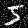
\includegraphics[width=2cm]{mnist/noisy}};
				\draw [|->] (0, 0) -- (1.0, 0);
				\node at (1.7, 0) {\( \begin{pmatrix}.2\\.1\\.2\\.2\\.3\end{pmatrix} \)};
			\end{scope}
			\node at (.0, -4) {Classification};
		\end{scope}
		\begin{scope}[xshift=5.3cm]
			\node at (0.5, 2.4) {\( f_{n}(\,\cdot\,,\Theta_{n}) : \)};
			\node at (-1.4, 1.7) {\( \mathbb{R}^{28 \times 28} \)};
			\node at (2.4, 1.7) {\(  \mathbb{R}^{28 \times 28} : \)};
			\draw [->] (0, 1.7) -- ++(1., 0);
			\draw [|->] (0, 0) -- ++(1., 0);
			\node at (-1.3, 0) {
\includegraphics[width=2cm]{mnist/00}};
			\node at (2.4, 0) {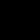
\includegraphics[width=2cm]{mnist/nonoise}};
			\begin{scope}[yshift=-2.5cm]
				\node at (-1.3, 0) {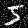
\includegraphics[width=2cm]{mnist/noisy}};
				\node at (2.4, 0) {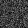
\includegraphics[width=2cm]{mnist/noise}};
				\draw [|->] (0, 0) -- ++(1., 0);
			\end{scope}
			\fill [gray] (-2.95, -4.3) rectangle ++(.1, 6.8);
			\node at (.5, -4) {Noise estimation};
		\end{scope}
		\begin{scope}[xshift=11.8cm]
			\node at (0.5, 2.4) {\( f_{l}(\,\cdot\,,\Theta_{l}) : \)};
			\node at (-1.3, 1.7) {\( \mathbb{R}^{28 \times 28} \)};
			\node at (1.7, 1.7) {\(  \mathbb{R} : \)};
			\draw [->] (0, 1.7) -- ++(1., 0);
			\draw [|->] (0, 0) -- ++(1., 0);
			\node at (-1.3, 0) {
\includegraphics[width=2cm]{mnist/00}};
			\node at (1.7, 0) {4.5};
			\begin{scope}[yshift=-2.5cm]
				\node at (1.7, 0) {1.3};
				\node at (-1.3, 0) {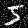
\includegraphics[width=2cm]{mnist/noisy}};
				\draw [|->] (0, 0) -- ++(1., 0);
			\end{scope}
			\fill [gray] (-2.85, -4.3) rectangle ++(.1, 6.8);
			\node at (.0, -4) {Likelihood estimation};
		\end{scope}
	\end{tikzpicture}
	\caption[Example applications of neural networks]{%
		Examples of neural networks:
		In the five-class classification problem on the left, the neural network \( f_c(\argm, \Theta_c) \) maps from the input space, images of size \numproduct{28x28} with real pixels, to the five-dimensional unit simplex.
		The entries of a vector which is an element of the five-dimensional unit simplex can be interpreted as probabilities.
		The goal here is (loosely speaking) that the correct class (here class \enquote{5}) has the highest probability.
		In the noise estimation problem in the middle, the neural network \( f_n(\argm, \Theta_n) \) maps from the input space to itself;
		An estimate of a noise-free image could be given by subtracting the output of the neural network from the input.
		In the likelihood estimation problem on the right, the neural network \( f_l(\argm, \Theta_l) \) maps from the input space to the real line.
		Here, the real number that is assigned to an input reflects its likelihood under the learned model.
		Although the noise- and likelihood estimation problem seem unrelated, there is an extremely close connection via Tweedie's identity.
		We discuss this in more detail in~\cref{chap:pogmdm}.
	}%
	\label{fig:neural network examples}
\end{figure*}

We now explore the \emph{architecture} of \glspl{nn}, recalling some concepts needed later.
A \gls{nn} \( f \) typically consists of a cascade of composed functions.
Specifically, an \emph{\( L \)-layer network} is structured as
\begin{equation}
	f = f_L \composed f_{L-\num{1}} \composed \cdots \composed f_{\num{2}} \composed f_{\num{1}}.
	\label{eq:neural network composition}
\end{equation}
Each layer \( \map{f_i}{\mathcal{X}_{i-\num{1}} \times \Theta_i}{\mathcal{X}_{i}} \) for \( i = \num{1}, \dotsc, L \) can be decomposed into a linear map followed by a point-wise non-linearity, and typically has its own parameters in the parameter space \( \Theta_i \subseteq \Theta \).\footnote{%
	We say subset of or equal to because the \gls{nn} may only have one parametrized layer.
}
An \( L \)-layer network is often referred to as having a \emph{depth} of \( L \), with all layers between the input and the output considered \emph{hidden}.

In the next section, we provide more detail on the linear and non-linear elements that constitute a layer.
Specifically, within the context of image processing, we explore \emph{convolutional layers} and some of the most popular nonlinearities.
The architectures and building blocks we use in this thesis are relatively straightforward.
For a more comprehensive review, see Cong and Zhou's survey~\cite{Cong2022}.
\subsection{Linear layers}
The linear sub-layers in \glspl{nn} are general affine maps.
Formally, let \( \mathcal{X}_l \) and \( \mathcal{X}_{l+1} \) represent the input and output spaces of layer \( f_l \).
The linear sub-layer within \( f_l \) is the affine map
\begin{equation}
	\mathcal{X}_l \times \Theta_l \ni (x, \theta) \mapsto K_lx + b_l
\end{equation}
where \( \map{K_l}{\mathcal{X}_l}{\mathcal{X}_{l + \num{1}}} \) is an arbitrary linear operator, and \( b_l \in \mathcal{X}_{l + \num{1}} \) is the affine offset, commonly referred to as \emph{bias} in the \gls{nn} literature.
The parameters \( \theta_l \) could be all weights in \( K_l \) and entries in \( b_l \).
However, often \( K_l \) and \( b_l \) are derived from a much lower dimensional object.
For example, the operator \( K_l \) can model the convolution of the input with the convolution kernels encoded in the entries of \( \theta \).

This thesis considers two primary types of linear sub-layers:
dense and fully-learned operators, and convolution operators.
These are particularly relevant in imaging applications.
Dense linear operators are useful for \enquote{inverting} imaging transforms such as the Fourier or the Radon transform.
Conversely, convolutions are crucial due to their inherent translation equivariance which is often desired in imaging tasks.

Sub-layers employing dense, fully-learnable operators are typically called \emph{fully connected}.
Here, the learnable parameters are \emph{all} weights in \( K_l \) and entries in \( b \).
In imaging applications, this can be extremely memory intensive:
Consider an image \( x \) of size \( \Height \times \Width \) with three color channels, i.e., \( x \in \R^{\Height \times \Width \times \num{3}} \) and assume we want to learn a linear operator that maps from this space to itself.
This linear operator has \( (\Height \times \Width \times \num{3}) \times (\Height \times \Width \times \num{3}) \) weights.
For a \( \Height = \Width = \num{256} \) square image, this amounts to \num{38654705664} weights, requiring more than \qty{154}{\giga\byte} of storage as \num{32}-bit floating-point numbers.
We use a fully connected layer as the last layer in our deep neural regularizer discussed in~\cref{chap:deep neural regularizers}.
There, the output space is a scalar and consequently the number of learnable parameters in the fully connected layer is equal to the dimensionality of its input space.

In imaging applications, \emph{convolution layers} are especially important.
Unlike fully connected layers, not all weights in the linear operator are learnable.
Instead, the operator's weights are derived from a learnable \emph{kernel} and the operator is constructed to encode a convolution.
Let \( x \in \mathcal{X}_{l-\num{1}} = \R^{c_{l-\num{1}} \times \Height_{l-\num{1}} \times \Width_{l-\num{1}}} \) be the input the \( l \)-th layer of the \gls{nn}.
In image processing, \( c_{l-\num{1}} \in \mathbb{N} \) are \emph{features} or \emph{channels} of the (\( l - \num{1} \))-th layer.
If the \( l \)-th layer has \( c_l \) features, the linear operator is a map \( \map{K_l}{\R^{c_{l-\num{1}} \times \Height_{l-\num{1}} \times \Width_{l-\num{1}}}}{\R^{c_{l} \times \Height_{l-\num{1}} \times \Width_{l-\num{1}}}} \), i.e.\ the size of the features remains unchanged.
The application of the linear operator is described by a total of \( c_{l-\num{1}} c_l\) convolutions.
Formally, let \( k^l_{c, d} \in \R^{s \times s} \) be a kernel of size \( s \times s \) where \( \num{1} \leq c \leq c_{l-\num{1}} \) and \( \num{1} \leq d \leq c_{\num{1}} \).
Then, the application of the linear operator \( K_l \) is described by
\begin{equation}
	(K_l x)_{c, i, j} = \sum_{d=\num{1}}^{c_{l-\num{1}}} \sum_{a,b=\num{1}}^{s,s} (k^l_{c, d})_{a, b} \cdot x_{d, \operatorname{bdy}(i - a + \lfloor s / \num{2} \rfloor, \Height_{l-1}), \operatorname{bdy}(j - b + \lfloor s / \num{2} \rfloor, \Width_{l-\num{1}})}.
\end{equation}
Here, the map \( \map{\operatorname{bdy}}{\mathbb{N} \times \mathbb{N}}{\mathbb{N}} \) can be used to realize different boundary conditions when \( \num{0} < i - a + \lfloor s / \num{2} \rfloor \leq \Height_{l-\num{1}} \) or \( \num{0} < j - b + \lfloor s / \num{2} \rfloor \leq \Width_{l-\num{1}} \) do not hold, see~\cref{ssec:convolutions}.
In the context of this thesis, the most important technique is \emph{periodic} or \emph{circular} boundary handling due to its relations with the Fourier transform.
There, the signals are assumed to be \( (\Height_{l-\num{1}}, \Width_{l-\num{1}}) \)-periodic, i.e.\ \( \operatorname{bdy} \) is given by\footnote{%
	This is written in array-notation with one-based indexing.
	A more familiar form is simply \( a \mod b \) for sequence-notation with zero-based indexing.
}
\begin{equation}
	(a, b) \mapsto (a + (b - \num{1}) \mod b) + \num{1}.
\end{equation}
In this case, we can make use of the \emph{convolution theorem} to diagonalize the linear operator \( K_l \) using the Fourier transform, see~\cref{chap:pogmdm}.

To expand the receptive field of subsequent layers, neural networks often integrate \emph{downsampling} layers.
It suffices to describe the action of downsampling layers on one channel; the application to multiple channels is channel-wise.
Applying a \( d \)-fold downsampling layer to an image of size \( \Height \times \Width \) results in an output image of size \( \frac{\Height}{d} \times \frac{\Width}{d} \) as illustrated in~\cref{fig:downsampling}.
There, every \( d \)-th pixel is copied into the output and consequently downsampling layers have no learnable parameters.
\begin{sidefigure}
	\centering
	\begin{tikzpicture}[every node/.style={anchor=center,inner sep=0, thick, draw, minimum size=5mm},]
		\matrix [matrix of nodes,column sep=0mm,row sep=0mm] (input)
		{
			\textcolor{maincolor}{8} & 1 & \textcolor{maincolor}{6} & 8 \\
			3 & 5 & 7 & 9 \\
			\textcolor{maincolor}{4} & 9 & \textcolor{maincolor}{2} & 5 \\
			9 & 4 & 5 & 6 \\ 
		};
		\matrix [below=of input, matrix of nodes,column sep=0mm,row sep=0mm]
		{
			\textcolor{maincolor}{8} & \textcolor{maincolor}{6} \\
			\textcolor{maincolor}{4} & \textcolor{maincolor}{2} \\
		};
	\end{tikzpicture}
	\caption[Action of a downsampling layer]{Visualization of a \num{2}-fold downsampling operation.}
	\label{fig:downsampling}
\end{sidefigure}
A practical implementation of downsampling involves merging convolution and downsampling operations into \emph{strided convolutions}, minimizing unnecessary computations.
\subsection{Nonlinearities}
\label{ssec:nonlinearities}
Composing only linear layers would result in an overall linear function, which is insufficient for many tasks and famously fails to solve the \enquote{XOR} problem.
Thus, in order for the composition~\cref{eq:neural network composition} to become any stronger than linear, the layers must incorporate nonlinearities.

Nonlinearities in \glspl{nn} typically act point-wise.
Formally, assume that the linear sub-layer in the \( l \)-th layer (which is not the output layer) maps to \( \tilde{\mathcal{X}}_l = \R^{f_l \times \Height_l \times \Width_l} \).
The nonlinear sub-layer is a function \( \map{\Phi_l}{\tilde{\mathcal{X}}_l}{\tilde{\mathcal{X}}_l} \) often structured such that it applies the same function \( \map{\phi_l}{\R}{\R} \) point-wise:
\begin{equation}
	\bigl(\Phi_l(x)\bigr)_{i, j, k} = \phi_l(x_{i, j, k})
	\label{eq:shared pointwise nonlinearity}
\end{equation}
and often the scalar function \( \phi_l \) is also shared between all layers.
The output space of the \( i \)-th nonlinear sub-layer is the input space of the (\( i + \num{1} \))-th layer, i.e., \( \mathcal{X}_{i + \num{1}} = \tilde{\mathcal{X}}_l \).

Numerous activation functions have been proposed in the literature;
for a relatively recent and comprehensive overview see~\cite{dubey_activation_2022}.
Popular examples include the logistic sigmoid \( x \mapsto (\num{1} + \exp(-x))^{\num{-1}} \) and the hyperbolic tangent \( x \mapsto \frac{\exp(x) - \exp(-x)}{\exp(x) - \exp(-x)} \).
However, these suffer from vanishing or exploding gradients.
The rectified linear unit \( \relu = (x \mapsto \max(\num{0}, x)) \) has become a favored choice to mitigate this.
While \( \relu \) is not differentiable at \( \num{0} \), automatic differentiation frameworks such as PyTorch~\cite{paszke_pytorch_2019}, handle this by choosing an element of the subdifferential at \( \num{0} \), usually \( \num{0} \).
However, an implicit differentiation framework that encompasses nonsmooth functions has been missing until relatively recently.
In 2021, Bolte et al. introduced the notion of \emph{path differentiability} in~\cite{bolte_nonsmooth_implicit_2021} which aims to resolve this problem.

The nondifferentiability of \( \relu \) poses a challenge for classical optimization algorithms.
We optimize our learned networks (w.r.t.\ their input) in~\cref{chap:deep neural regularizers} with standard first-order optimization methods discussed in~\cref{ssec:nonconvex optimization}.
While optimization works well empirically, we can not guarantee convergence.
Surrogates for \( \relu \) such as the swish \( x \mapsto \frac{x}{\num{1} + \exp(-x)} \) or the exponential linear unit
\[
	x \mapsto \begin{cases}
		x &\ \text{if}\ x > \num{0}, \\
		\exp(x) - \num{1} &\ \text{else},
	\end{cases}
\]
offer differentiable alternatives.
If one wants to avoid the computational complexity of these functions during training but ensure convergence of optimization algorithms, it is possible to replace the rectified linear activation functions with a differentiable counterpart after training.
However, in order for the learned parameters to be meaningful, the surrogate must approximate \( \relu \) well, and the gradient of any reasonable approximation will necessarily have an exploding Lipschitz constant, effecting optimization speed.

In~\cref{chap:regularizers} we use a \emph{leaky} rectified linear activation given by
\begin{equation}
	\relu = x \mapsto \max(\gamma x, x)
\end{equation}
with the small leakage coefficient \( \gamma > \num{0} \).
The discussion about nondifferentiability, its implications, and possible remedies carries over to this version.
\Cref{fig:nonlinearities} showcases a selection of popular nonlinearities.
\begin{sidefigure}
	\begin{tikzpicture}[declare function={
		lrelu(\x,\g)=max(\g*\x, \x);
		elu(\x)=(x > 0) * x + (x < 0) * (exp(x) - 1);
		swish(\x)=\x/(1 + exp(-\x));
		sigmoid(\x)=1/(1 + exp(-\x));
	}]
		\begin{axis}[domain=-2:2, marginplot, xmin=-2, xmax=2, no markers]
			\addplot+ [thick] {elu(x)};
			\addplot+ [thick] {lrelu(x, 0)};
			\addplot+ [thick] {lrelu(x, 0.1)};
			\addplot+ [thick] {swish(x)};
			\addplot+ [thick] {sigmoid(x)};
		\end{axis}
	\end{tikzpicture}
	\caption[Common nonlinearities in neural networks]{%
		\tikzexternaldisable
		Common nonlinearities in neural networks:
		The exponential linear unit %
		\protect\tikz[baseline=-\the\dimexpr\fontdimen22\textfont2\relax]\protect\draw [index of colormap={0} of flare, thick] (0,0) -- (.5, 0);,
		the rectified linear unit %
		\protect\tikz[baseline=-\the\dimexpr\fontdimen22\textfont2\relax]\protect\draw [index of colormap={4} of flare, thick] (0,0) -- (.5, 0); %
		and its leaky variant %
		\protect\tikz[baseline=-\the\dimexpr\fontdimen22\textfont2\relax]\protect\draw [index of colormap={8} of flare, thick] (0,0) -- (.5, 0);, %
		the swish %
		\protect\tikz[baseline=-\the\dimexpr\fontdimen22\textfont2\relax]\protect\draw [index of colormap={12} of flare, thick] (0,0) -- (.5, 0);, %
		and the sigmoid %
		\protect\tikz[baseline=-\the\dimexpr\fontdimen22\textfont2\relax]\protect\draw [index of colormap={17} of flare, thick] (0,0) -- (.5, 0);.
		\tikzexternalenable
	}%
	\label{fig:nonlinearities}
\end{sidefigure}

The choice of nonlinearity in the output layer depends on the task and is not necessarily point-wise.
For instance, in \( K \)-class classification problems, the soft-argmax\footnote{%
	This is sometimes given the misleading name \enquote{softmax}.
	However, it smoothly approximates the argmax function, not the maximum.
}
\begin{equation}
	\R^K \ni (x_{\num{1}}, \dotsc, x_K) \mapsto \begin{pmatrix}
		\frac{\exp(x_i)}{\sum_{i=\num{1}}^K\exp(x_i)}\\
		\vdots\\
		\frac{\exp(x_i)}{\sum_{i=\num{1}}^K\exp(x_i)}
	\end{pmatrix}.
\end{equation}
is a popular choice.
It maps any point onto the \( K \)-dimensional unit simplex \( \Simplex^K \) and hence its output values can be interpreted as probabilities.
Depending on the application, the identity map \( x \mapsto x \) may be suitable, making the output of the network the output of the last linear sub-layer.

The models we discuss in~\cref{chap:pogmdm} can be viewed as one-layer networks, with each of the \( \NumExperts \in \mathbb{N} \) convolution operators equipped with their own scalar-valued activation function.
Thus, \( \Phi \) has the block structure
\begin{equation}
	\R^{\Height \times \Width \times \NumExperts} \ni (x_{\num{1}}, \dotsc, x_{\NumExperts}) \mapsto (\Phi_{\num{1}}(x_{\num{1}}), \dotsc, \Phi_\NumExperts(x_\NumExperts))
\end{equation}
where each \( \map{\Phi_i}{\R^{m \times n}}{{\R^{m\times n}}} \) shares the same \( \map{\phi_i}{\R}{\R} \) across all \( i = \num{1}, \dotsc, \NumExperts \).
The nonlinearities are log-sum-exp functions, interpreted as the negative logarithm of a probability density function parametrized through a \gls{gmm}.
Thus, the nonlinearities are endowed with parameters that we \emph{learn} from data.
\section{Supervised and unsupervised learning}
Machine learning approaches are classically divided into \emph{supervised learning} and \emph{unsupervised learning}~\cite{bishop_pattern_2006}.
In this section, we elaborate on the differences between these two approaches.

In \emph{supervised learning}, we are given a reference dataset of (input, output) pairs, and the goal is to learn a parametric map that accurately reproduces the reference output for a given input.
Formally, consider a pair \( (X, Y) \) of random variables, where \( Y \) is the input random variable with values in \( \mathcal{Y} \), and \( X \) is the output random variable with values in \( \mathcal{X} \).
Here, we adopt the notation from the introduction and the rest of the thesis which is in contrast to the previous section; there the input and output spaces are flipped.
We assume that the pair \( (X, Y) \) is distributed as \( p_{X, Y} \).

The objective is to learn a parametric map
\begin{equation}
	\map{f}{\mathcal{Y} \times \Theta}{\mathcal{X}}
\end{equation}
that maps an input \( y \in \mathcal{Y} \) to \( f(y, \theta) \in \mathcal{X} \) given parameters \( \theta \in \Theta \).
The set of admissible parameters \( \Theta \) can encode constraints on the parameter vector \( \theta \), e.g.\ to enforce invariances.
To find optimal parameters, we minimize a loss function \( \map{l}{\mathcal{X} \times \mathcal{X}} \) that compares two points in the output space \( \mathcal{X} \):
\begin{equation}
	\min_{\theta \in \Theta}\Expectation_{(X, Y)\sim p_{X,Y}}\bigl[ l(f(Y, \theta), X) \bigr].
\end{equation}

Supervised learning encompasses classification, where the output space is discrete, and regression, where the output space is continuous.
Examples of the former include classification problems in computer vision, such as semantic segmentation or object detection, but also problems like spam detection or bot detection.
Examples of the latter include polynomial regression, stock price prediction, and image reconstruction.

In \emph{unsupervised learning}, we aim to find structure in the distribution of the \emph{input} random variable \( Y \).
A prototypical example is \emph{density estimation}, which aims to fit a parametric model to the density of the random variable.
This is often formalized as maximum likelihood learning, which amounts to finding parameters \( \theta \) of a parametric density \( \map{p}{\mathcal{Y} \times \theta}{\interval{\num{0}}{\infty}} \) via
\begin{equation}
	\min_{\theta \in \Theta} \Expectation_{Y \sim \DensityFunction_Y}\bigl[ -\log p(Y, \theta) \bigr].
\end{equation}
\begin{sidefigure}
	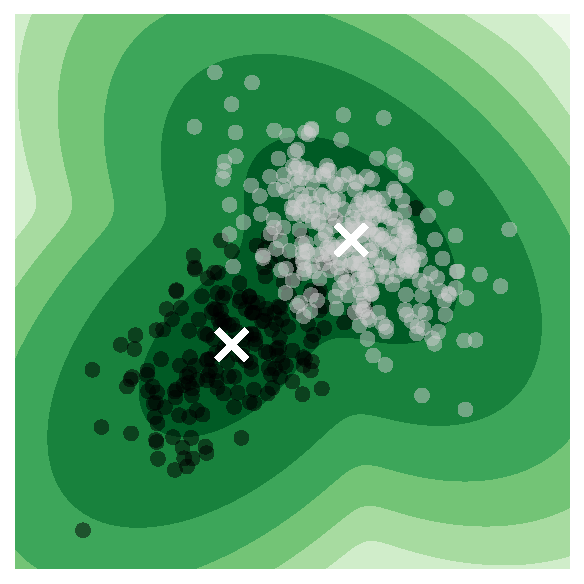
\includegraphics[width=\marginparwidth]{learning-types/gmm}
	\caption[Unsupervised learning: Density estimation]{
		Density estimation of a point cloud with a Gaussian mixture model.
		The white crosses indicate the means of the two components and the shades of green indicate the density.
	}%
	\label{fig:unsupervised gmm}
\end{sidefigure}

Another classic unsupervised task is \emph{clustering}, where the aim is to partition the input space into disjoint regions based on an unlabeled dataset.
A query point can then be assigned to one of the clusters based on its region.
Fixing the number of clusters to \( K \) and constructing the disjoint regions such that the Euclidean distance between points in the regions is minimized leads to the famous \( K \)-means algorithm~\cite{lloyd_least_1982}.
\begin{sidefigure}
	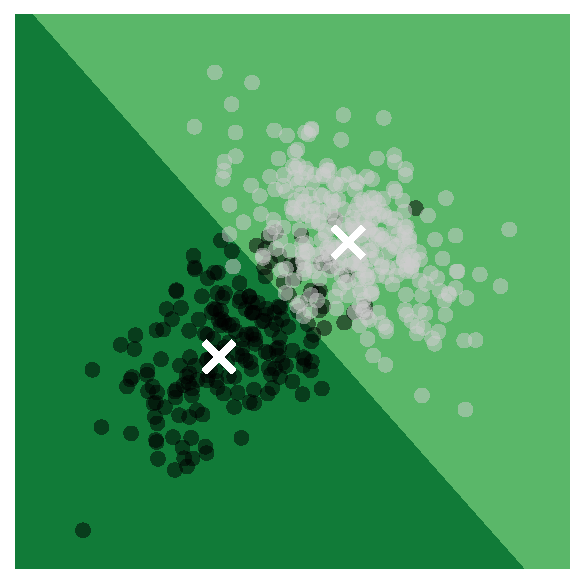
\includegraphics[width=\marginparwidth]{learning-types/km}
	\caption[Unsupervised learning: Clustering]{
		Clustering of a point cloud with K-means.
		The white crosses indicate the centroids of the two clusters and the shades of green indicate the cluster a point is assigned to.
	}%
	\label{fig:unsupervised km}
\end{sidefigure}
\Cref{fig:unsupervised gmm} and \cref{fig:unsupervised km} show examples of density estimation with a Gaussian mixture model and clustering with the K-means algorithm on a point cloud drawn from two Gaussians in two dimensions.
\section{Generative and discriminative learning}
This thesis focuses on using \emph{generative learning} for inverse problems in imaging.
Here, we distinguish between generative and discriminative learning by considering a supervised estimation problem.
Consider a pair of random variables \( (X, Y) \) with joint distribution \( p_{X, Y } \) and marginal distributions \( p_X \) and \( p_Y \).
As in the previous section, \( Y \) is the \emph{input} random variable and \( X \) is the output random variable.

In the \emph{discriminative approach}, the joint distribution is factorized as
\begin{equation}
	p_{X, Y} = p_{X\mid Y} p_Y,
\end{equation}
where \( p_{X\mid Y} \) is the \emph{posterior} of the output given the input and \( p_Y \) is the density of the input.
Training parametric estimators of this type\footnote{%
	in the standard maximum-likelihood framework; the conclusions also hold for more general formulations.
} amounts to finding
\begin{equation}
	\min_{\theta_{X \mid Y}, \theta_Y} \Expectation_{(X, Y) \sim p_{X, Y}}\bigl[ -\log \hat{p}_{X\mid Y}(X, Y, \theta_{X\mid Y}) \bigr] + \Expectation_{Y \sim p_Y} \bigl[ -\log \hat{p}_Y(Y, \theta_Y) \bigr],
\end{equation}
where  \( \hat{p}_{X\mid Y}(\argm,\argm,\theta_{X\mid Y}) \) and \( \hat{p}_Y(\argm, \theta_Y) \) are parametric estimators.
Thus, the discriminative approach decouples into the posterior and the input density.

For practical inference problems, the parametric posterior suffices:
Given an input \( y \in \mathcal{Y} \), the associated estimation of the output can be found via\footnote{For the sake of simplicity, we only discuss \gls{map} estimation}
\begin{equation}
	\argmax_{x \in \mathcal{X}} \hat{p}_{X \mid Y} (x, y, \theta_{X \mid Y}).
\end{equation}
The discriminative approach has the advantage that the parametric posterior is typically simpler than the density of the output; see the example below.
However, it is challenging to encode domain knowledge and it is typically impossible to adapt to changes in the relationship between the input and output random variables;
we demonstrate this with an example in \gls{mri} in~\cref{sec:discriminative pitfalls}.

In the \emph{generative approach}, the joint distribution is factorized as
\begin{equation}
	p_{X, Y} = p_{Y \mid X} p_X,
\end{equation}
where \( p_{Y \mid X} \) is the \emph{likelihood} of an input given an output, and \( p_X \) is the density of the output.
Training parametric estimators of this type amounts to finding
\begin{equation}
	\min_{\theta_{Y \mid X}, \theta_X} \Expectation_{(X, Y) \sim p_{X, Y}}\bigl[ -\log \hat{p}_{Y\mid X}(X, Y, \theta_{Y\mid X}) \bigr] + \Expectation_{X \sim p_X} \bigl[ -\log \hat{p}_X(X, \theta_X) \bigr],
\end{equation}
where \( \hat{p}_{Y \mid X}(\argm, \argm, \theta_{Y\mid X}) \) and \( \hat{p}_X(\argm, \theta_X) \) are parametric estimators.
When the parameters are learned, we can invoke Bayes theorem and write the posterior as
\begin{equation}
	\hat{p}_{X \mid Y} = \frac{\hat{p}_{Y \mid X}(\argm, \argm, \theta_{Y \mid X})\hat{p}_X(\argm, \theta_X)}{\hat{p}_Y}
\end{equation}
where the denominator is irrelevant with respect to the inference
\begin{equation}
	\argmax_{x \in \mathcal{X}} \hat{p}_{Y\mid X}(x, y, \theta_{Y \mid X}) \hat{p}_X(x, \theta_X).
\end{equation}
Thus, the generative approach separates the input likelihood from the output prior and invokes Bayes theorem for the posterior.

In this thesis, the likelihood is determined by the physical acquisition model and has extremely few parameters\footnote{usually one: the noise variance}, identified through grid search on a validation dataset.
Thus, the likelihood of \( Y \) given \( X \) is \emph{known, easy to model, and subject to change}.
Therefore, a generative learning approach is advantageous, as it allows for easy encoding of domain knowledge in the likelihood.
In addition, changes to the likelihood only require retraining of the parametric likelihood \( -\log \hat{p}_{Y \mid X}(\argm, \argm, \theta_{Y \mid X}) \).

In this taxonomy, \emph{supervised and unsupervised} as well as \emph{generative and discriminative} are understood with respect to the downstream task.
For example, in~\cref{chap:deep neural regularizers}, we learn a parametric form of the density of \gls{mri} images of the human knee.
For image reconstruction, this learned density represents the density of the \emph{output} random variable, making the approach \emph{generative} because it separates the input likelihood from the output prior.
However, it is \emph{supervised} because we train on the density of the output random variable.
For pathology detection\footnote{%
	With the learned density, pathology detection could for instance be implemented via simple likelihood evaluation.
}, this approach is \emph{unsupervised} (because there are no labels) but not generative:
Generative learning would amount to learning the density of the output random variable (essentially a scalar representing the pathologies prevalence), as well as the class conditional densities of images with and without pathologies.

We emphasize that discriminative learning is typically easier than generative learning through a two-class classification problem:
Assuming two normally distributed random variables with arbitrary mean and covariance, discriminative methods derive a parametric form of the posterior class density given a query point.
This object can famously be represented\footnote{%
	For either class; the posterior density for the other is just one minus the object.
} as (see, e.g.~\cite[section 4.2.1.]{bishop_pattern_2006})
\begin{equation}
	x \mapsto \bigl( \num{1} + \exp(\inprod{x}{Ax} + \inprod{b}{x} + c) \bigr)^{\num{-1}},
\end{equation}
where \( A \), \( b \), and \( c \) are a symmetric matrix, vector, and scalar, respectively.
For determining the most likely class, this simplifies further to identifying the parameters defining the hyperbolic decision boundary (depicted as a white line in~\cref{fig:discriminative}).
\begin{sidefigure}
	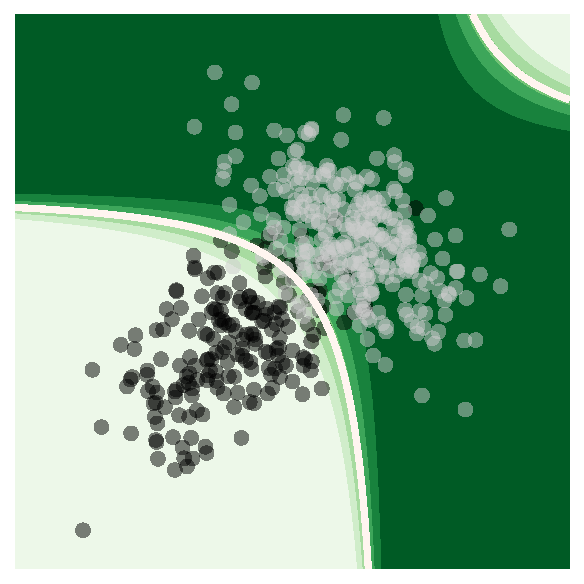
\includegraphics[width=\marginparwidth]{learning-types/discriminative}
	\caption[Discriminative two-class classification]{%
		Discriminative approach to the two-class classification problem:
		Darker green indicates higher posterior values of belonging to the \enquote{white} class.
		The white line is the hyperbolic decision boundary.
	}%
	\label{fig:discriminative}
\end{sidefigure}
In contrast, generative modeling finds the two class-conditional distributions, both general normal distributions, along with the class priors.
This requires estimating two symmetric positive definite matrices, two mean vectors and a scalar representing the class priors.
This is illustrated in~\cref{fig:generative}, where level lines are related to the covariance matrices and the size of the cross indicating the means is related to the class prior.
A new point is then classified according to its weighted likelihood.
\begin{sidefigure}
	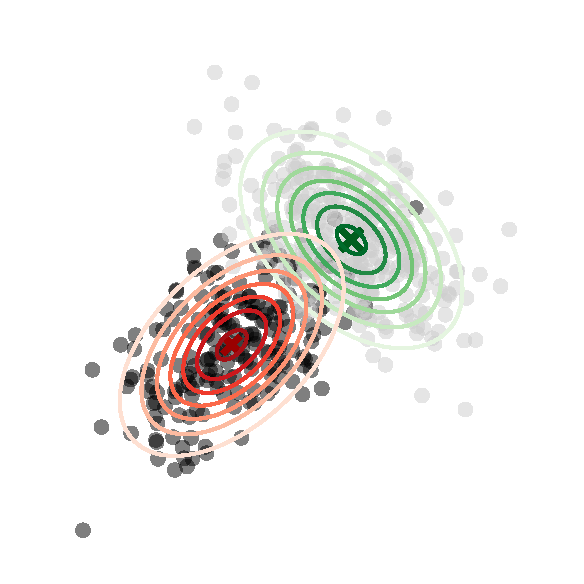
\includegraphics[width=\marginparwidth]{learning-types/generative}
	\caption[Generative two-class classification]{
		Generative approach to the two-class classification problem:
		The level lines are related to the covariance matrices, the size of the cross markers indicating the mean is related to the prior probability of a class.
		New points are classified according to the weighted likelihood; the decision boundary is shown in~\cref{fig:discriminative}.
	}%
	\label{fig:generative}
\end{sidefigure}

In the above example, the challenge lied mostly in finding the likelihood densities.
In this case, (for the purpose of pure classification) there is not merit to the generative approach.
However, in the inverse problems in imaging considered in this thesis, the likelihood of an input given an output is fixed by the physical acquisition model and is parameter-free up to scaling.
In addition, the physical acquisition model is subject to change:
As an example, in~\cref{chap:deep neural regularizers} we consider different frequency selections in a Fourier imaging setup.
On the other hand, the prior distribution of images is an extremely complicated object.
Thus, in this case the generative approach proves beneficial.
\Cref{chap:deep neural regularizers,chap:pogmdm} discuss two methods for learning a parametric density of image priors, highlighting the applicability of generative learning in such contexts.
